\documentclass{amsart}
\usepackage{mathtools}
\usepackage{tikz}
\usepackage{subcaption}
\usepackage[dutch]{babel}
\usepackage[T1]{fontenc}
\usetikzlibrary{arrows.meta}

%%% ENV

\tikzset{>=Stealth}
\tikzstyle{vector}=[->,thick,black]

\theoremstyle{definition}
\newtheorem{axm}{Axioma}[section]
\newtheorem{thm}{Stelling}[section]
\newtheorem{lmm}{Lemma}[section]
\newtheorem{dfn}{Definitie}[section]
\newtheorem{csq}{Gevolg}[section]

\newenvironment{bewijs}{\begin{proof}[Bewijs]}{\end{proof}}

%%% CMD

%% sets

\newcommand{\setsm}[1]{\{{#1}\}}
\newcommand{\without}[1]{\setminus\setsm{#1}}
\newcommand{\with}[1]{\cup\setsm{#1}}

\newcommand{\realnums}{\mathbb{R}}
\newcommand{\realn}[1][n]{\realnums^{#1}}
\newcommand{\realmx}[2][n]{\realn[#2 \times #1]}
\newcommand{\realnxn}{\realmx{n}}
\newcommand{\realmxn}{\realmx{m}}

\newcommand{\vecspace}[1][v]{\mathrm{\mathbf{\MakeUppercase#1}}}
\newcommand{\vecspacen}[1][n]{\vecspace^#1}


%% numbers

\newcommand{\norm}[1]{\lVert{#1}\rVert}
\newcommand{\abs}[1]{\lvert{#1}\rvert}


%% vectors

% bold vectors
\newcommand{\vvec}[1][v]{\mathbf{#1}}
\newcommand{\uvec}[1][v]{\vvec[#1]_\mathbf{e}}

\newcommand{\vnorm}[1]{\norm{\vvec[#1]}}
\newcommand{\zerovec}{\vvec[0]}

% vector rows and their vectors
\newcommand{\vecrow}[1][a]{\mathfrak{\MakeUppercase{#1}}}

\newcommand{\rvec}[2][i]{{#2}_{#1}}
\newcommand{\rvecr}[2][i]{\rvec[#1]{\vecrow[#2]}}
\newcommand{\rveci}[1][i]{\rvecr[#1]{a}}

% coordinate vectors
\newcommand{\cvec}[2]{{#1}^{#2}}

\newcommand{\cveca}[2][a]{\cvec{#2}{\vecrow[#1]}}

\newcommand{\cvecv}[2][v]{\cvec{\vvec[#1]}{#2}}
\newcommand{\cvecva}[1][a]{\cvecv{\vecrow[#1]}}
\newcommand{\cvecc}[2][a]{\cvecv[#2]{\vecrow[#1]}}
\newcommand{\cvecvv}[1][v]{\cvecc{#1}}

% coordinates
\newcommand{\vcord}[3]{{#1}_{#2}^{#3}}

\newcommand{\vcorda}[3][a]{\vcord{#2}{#3}{\vecrow[#1]}}
\newcommand{\vcordai}[2][i]{\vcorda{#2}{#1}}

\newcommand{\vcordv}[3][v]{\vcord{#1}{#2}{\vecrow[#3]}}
\newcommand{\vcordvi}[2][i]{\vcordv{#1}{#2}}

\newcommand{\vcordvia}[1][i]{\vcordvi[#1]{a}}


%%% DOC

\begin{document}
\title{Lineaire algebra}
\author{Olesj Bilous}
\maketitle

\section{Vectorruimtes}


\begin{dfn}
    Een vectorruimte $\vecspace$ bevat van elke vector $\vvec \in \vecspace$ een unieke schaal $\lambda \vvec$ voor elke scalair $\lambda \in \realnums$. Het bevat ook de unieke som $\vvec + \vvec[w]$ van elk paar vectoren $\vvec, \vvec[w] \in \vecspace$.
\end{dfn}

\begin{axm}
    De vectorschaal is associatief.
    \begin{equation*}
        \lambda (\mu \vvec) = (\lambda\mu)\vvec
    \end{equation*}
\end{axm}

\begin{axm}
    $1\vvec$ is de identiteitsschaal.
    \begin{equation*}
        1\vvec=\vvec
    \end{equation*}
\end{axm}

\begin{axm}
    Er bestaat een unieke nulvector $\zerovec$ die de nulschaal is van elke vector $\vvec \in \vecspace$.
    \begin{equation*}
        0\vvec=\zerovec
    \end{equation*}
\end{axm}

\begin{axm}
    De vectorsom is associatief.
    \begin{equation*}
        (\vvec[u] + \vvec) + \vvec[w] = \vvec[u] + (\vvec + \vvec[w])
    \end{equation*}
\end{axm}

\begin{axm}
    De vectorsom is commutatief.
    \begin{equation*}
        \vvec + \vvec[w] = \vvec[w] + \vvec
    \end{equation*}
\end{axm}

\begin{axm}
    De vectorschaal is distributief over de vectorsom.
    \begin{equation*}
        \lambda(\vvec + \vvec[w]) = \lambda \vvec + \lambda \vvec[w]
    \end{equation*}
\end{axm}

\begin{axm}
    De vectorschaal is distributief over de scalaire som.
    \begin{equation*}
        (\lambda + \mu)\vvec = \lambda \vvec + \mu \vvec
    \end{equation*}
\end{axm}

\begin{thm}
    Een vectorruimte is een commutatieve groep over de vectorsom.
    \begin{bewijs}
        \begin{align*}
            \vvec + 0\vvec    & = (1+0)\vvec \\
            \vvec + (-1)\vvec & = (1-1)\vvec
        \end{align*}
    \end{bewijs}
\end{thm}

\begin{figure}
    \def\vx {3}
    \def\vy {0}
    \def\wx {-1.5}
    \def\wy {2.2}
    \centering
    \begin{subcaptionblock}{.4\textwidth}
        \centering
        \begin{tikzpicture}
            \def\vscale{1.7}
            \def\vsmall{1.7}
            \def\dxsmall{0.3}
            \def\dysmall{1}
            \def\circum{2pt}
            \def\lower{-0.7}
            \def\sol{0}
            \def\ooscale
            {
                -\lower
            }

            \coordinate (O) at (0,0);
            \coordinate (P) at (\vsmall,0);
            \coordinate (M) at (-\vsmall, 0);
            \coordinate (Q) at (\vscale*\vsmall, 0);
            \coordinate (D) at (\dxsmall,\dysmall);
            \coordinate (OO) at (-\ooscale*\dysmall, \ooscale*\dxsmall);
            \coordinate (DD) at (-\ooscale*\dysmall + \dxsmall, \ooscale*\dxsmall + \dysmall);
            \filldraw[black] (O) circle (\circum) node[below]{$\mathbf 0$};
            \draw[vector] (O)--(P) node[midway, below]{$\mathbf v$};
            \draw[vector] (O)--(D) node[midway, left]{$\mathbf w$};
            \draw[vector, dashed] (O)--(M) node[midway, below]{$-\mathbf v$};
            \draw[vector, dashed] (P)--(Q) node[midway, below]{$\lambda\mathbf v$};
            \draw[|-|] (0, \lower)--(\vsmall,\lower) node[midway, below]{$1$} ;
            \node[below] (a) at (0, \lower) {$0$};
            \draw[|-|] (0, \lower)--(-\vsmall,\lower) node[midway, below]{$-1$};
            \draw[|-|] (0, 2*\lower)--(\vscale*\vsmall, 2*\lower) node[midway, below]{$\lambda$};
            \draw[|-|] (OO)--(DD) node[midway, left]{$1$};
        \end{tikzpicture}
        \caption{Begrensde rechtlijnige paden in dezelfde richting kunnen naar willekeur geschaald worden. Een negatief teken wijst op de terugkerende zin, de nulschaal op het pad dat nergens heen gaat.}
        \label{fig:rlpscale}
    \end{subcaptionblock}\hspace{1em}%
    \begin{subcaptionblock}{.4\textwidth}
        \centering
        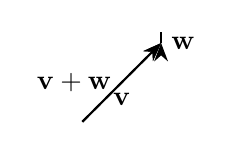
\begin{tikzpicture}
            \coordinate (O) at (0,0);
            \coordinate (P) at (\vx, \vy);
            \coordinate (R) at (\vx+\wx,\vy+\wy);
            \draw[vector]
            (O)--(P) node[midway, below]{$\mathbf v$};
            \draw[vector]
            (P)--(R) node[midway, right]{$\mathbf w$};
            \draw[vector,dashed]
            (O)--(R) node[midway, left]{$\mathbf{v + w}$};
        \end{tikzpicture}
        \caption{Een reis langs een rechtlijnig pad kan verdergezet worden langs een ander rechtlijnig pad. Er is telkens een rechtlijnig pad van de eerste oorsprong naar de laatste bestemming.}
        \label{fig:rlpcomp}
    \end{subcaptionblock}

    \begin{subcaptionblock}{.4\textwidth}
        \centering
        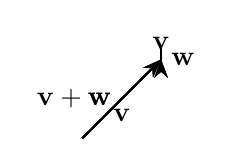
\begin{tikzpicture}
            \coordinate (O) at (0,0);
            \coordinate (P) at (\vx,\vy);
            \coordinate (Q) at (\wx, \wy);
            \coordinate (R) at (\vx+\wx,\vy+\wy);
            \draw[vector] (O)--(P) node[midway, below]{$\mathbf v$};
            \draw[vector] (Q)--(R) node[midway, above]{$\mathbf v$};
            \draw[vector] (P)--(R) node[midway, right]{$\mathbf w$};
            \draw[vector] (O)--(Q) node[midway, left]{$\mathbf w$};
            \draw[vector, dashed] (O)--(R) node[midway, left]{$\mathbf{v + w}$};
        \end{tikzpicture}
        \caption{De samenstelling van rechtlijnige paden is commutatief.}
        \label{fig:rlpcomm}
    \end{subcaptionblock}\hspace{1em}%
    \begin{subcaptionblock}{.4\textwidth}
        \centering
        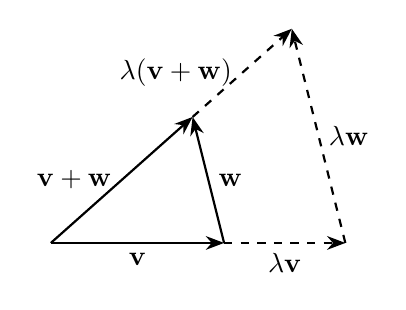
\begin{tikzpicture}
            \def\scale{1.7}
            \def\vxs{2.2}
            \def\wxs{-0.4}
            \def\wys{1.6}
            \coordinate (O) at (0,0);
            \coordinate (P) at (\vxs,0);
            \coordinate (R) at (\vxs+\wxs,\wys);
            \coordinate (PP) at (\scale*\vxs,0);
            \coordinate (RR) at (\scale*\vxs+\scale*\wxs,\scale*\wys);
            \draw[vector] (O)--(P) node[midway, below]{$\mathbf v$};
            \draw[vector] (P)--(R) node[midway, right]{$\mathbf w$};
            \draw[vector] (O)--(R) node[midway, left]{$\mathbf{v+w}$};
            \draw[vector, dashed] (P)--(PP) node[midway, below]{$\lambda\mathbf v$};
            \draw[vector, dashed] (PP)--(RR) node[midway, right]{$\lambda\mathbf w$};
            \draw[vector, dashed] (R)--(RR) node[midway, left]{$\lambda\mathbf{(v + w)}$};
        \end{tikzpicture}
        \caption{De schaal verdeelt over de samenstellende delen.}
        \label{fig:rlpdist}
    \end{subcaptionblock}
    \caption{De ruimte der rechtlijnige paden is een vectorruimte.}
\end{figure}

\begin{dfn}
    De nulruimte van een vectorruimte $\vecspace_0 = \setsm\zerovec \subseteq \vecspace$ bevat enkel de nulvector.
\end{dfn}

\begin{csq}
    De nulruimte is een triviale vectorruimte.
\end{csq}

\begin{csq}
    Een eindige deelverzameling van een vectorruimte is enkel een vectorruimte als het de triviale vectorruimte is.
\end{csq}

\begin{dfn}
    De lineaire combinatie van een rij vectoren $\rveci \in \vecrow \in \vecspacen$ volgens een kolom coëfficiënten $\vcordvia \in \cvecva \in \mathbb{R}^n$
    schaalt elke vector in de rij met de respectieve coëfficiënt in de kolom en somt over deze schalen.
    \begin{align*}
        \vecrow \cvecva
         & =
        \begin{pmatrix}
            \rveci[1], \ldots, \rveci[n]
        \end{pmatrix}
        \begin{pmatrix}
            \vcordvia[1] \\
            \vdots       \\
            \vcordvia[n]
        \end{pmatrix}
        \\ & = \sum_i^n \vcordvia \rveci
        \\ & = \vcordvia[1] \rveci[1] + \ldots + \vcordvia[n] \rveci[n]
    \end{align*}
\end{dfn}

\begin{csq}
    Zo is elke lineaire combinatie van vectoren $\rveci \in \vecspace$ ook een vector $\vecrow \cvecva = \vvec \in \vecspace$.
\end{csq}

\begin{dfn}
    De schaal van een kolom coëfficiënten $v_i \in \vvec \in \realn$ is de kolom $\vvec[w] \in \realn$ met de schalen van de respectieve coëfficiënten ${w}_i = \lambda {v}_i$.
    \begin{align*}
        \lambda \vvec =
        \lambda
        \begin{pmatrix}
            v_1    \\
            \vdots \\
            v_n
        \end{pmatrix}
        =
        \begin{pmatrix}
            \lambda v_1 \\
            \vdots      \\
            \lambda v_n
        \end{pmatrix}
    \end{align*}
\end{dfn}

\begin{dfn}
    De som van coëfficiëntkolommen $\vvec[u], \vvec \in \realn$ is de kolom $\vvec[w] \in \realn$ met de sommen van de respectieve coëfficiënten ${w}_i = {u}_i + {v}_i$.
    \begin{align*}
        \vvec[u] + \vvec =
        \begin{pmatrix}
            u_1    \\
            \vdots \\
            u_n
        \end{pmatrix}
        +
        \begin{pmatrix}
            v_1    \\
            \vdots \\
            v_n
        \end{pmatrix}
        =
        \begin{pmatrix}
            u_1 + v_1 \\
            \vdots    \\
            u_1 + v_n
        \end{pmatrix}
    \end{align*}
\end{dfn}

\begin{thm}
    $\realn$ is een vectorruimte met nulvector $0_n$ waar elke coëfficiënt nul is.
\end{thm}

Vandaar dat men een kolom coëfficiënten doorgaans een kolomvector zal noemen. De coëfficiënten heten dan componenten.

\begin{dfn}
    De vectorrij $A \in \realn[m \times n]$ met $n$ kolomvectoren $A_{j} \in \realn[m]$ noemt men een matrix.

    Evenwel vormt de matrix $A$ ook een vectorkolom met $m$ rijvectoren $A^i \in \realn$.

    De gemene component tussen $A_j$ en $A^i$ noemt men een element van de matrix, geschreven $a_{ij}$.
\end{dfn}

\begin{dfn}
    Transpositie $A^T \in \realmx[m]{n}$ spiegelt een matrix $A \in \realmxn$ om de diagonaal $a^T_{ij} = a_{ji}$ zodat rijen kolommen worden $(A^T)_j = (A^j)^T$ en vice versa.
\end{dfn}

\begin{csq}
    Herhaalde lineaire combinaties van een vectorrij $\vecrow \in \vecspacen[m]$ volgens de kolomvectoren $B_i$ van een matrix $B \in \realmxn$ vormen een vectorrij $\vecrow[b] \in \vecspacen$.
\end{csq}

\begin{dfn}
    Bovenstaande operatie noemen we de lineaire transformatie van $\vecrow$ volgens $B$.
    \begin{equation*}
        \vecrow B = \vecrow[b]
    \end{equation*}
\end{dfn}

\begin{dfn}
    De matrix die een vectorrij op zichzelf afbeeldt noemen we de identiteitsmatrix $I_n \in \realnxn$ zodat $\vecrow I_n = \vecrow$.

    Een kolom van deze matrix $s_j: \{i \in \mathbb N|i\leq n\}\longrightarrow\{0,1\}$ selecteert de respectieve vector uit de rij $\rveci[j]$ omdat het element $s_j(i) = 1$ enkel als $i = j$.
\end{dfn}

\begin{csq}
    De lineaire transformatie van de $m$ kolomvectoren $A_i \in \realn[k]$ van de matrix $A \in \realmx[m]{k}$ volgens de matrix $B \in \realmxn$ bestaat uit de $n$ kolomvectoren $C_j \in \realn[k]$ van de matrix $C \in \realmx[n]{k}$.
\end{csq}

\begin{dfn}
    Dit staat ook simpelweg als het matrixproduct bekend.
    \begin{equation*}
        AB = C
    \end{equation*}
\end{dfn}

\begin{csq}
    Elk van de $k$ rijvectoren $C^h \in \realn$ bestaat anderzijds uit een lineaire combinatie van $m$ rijvectoren $B^i \in \realn$ volgens de rijvector $A^h \in \realn[m]$, oftewel $(AB)^T = B^TA^T$.
\end{csq}

\begin{csq}
    Het matrixproduct is associatief $(AB)C = A(BC)$.
    \begin{bewijs}
        De vectorschaal is distributief over de vectorsom en bovendien associatief.
        Vandaar dat het in $ABC$ niet uitmaakt of een $C_i$ zijn coëfficiënten verdeelt over $AB$ of een $(BC)_j$ de zijne over $A$.
    \end{bewijs}
\end{csq}

\begin{csq}
    Inverteerbare vierkante matrices $A \in \realnxn$ zijn commutatief inverteerbaar.
    \begin{bewijs}
        Weze $AA^{-1}_r = I_n$ in $(AA^{-1}_r)A = A(A^{-1}_rA)$. Hierbij moet $A^{-1}_rA$ echter ook dezelfde identiteitsmatrix $I_n$ zijn.
    \end{bewijs}
\end{csq}

\begin{dfn}
    De spanruimte $span(\vecrow)$ van een vectorrij $\vecrow$ bevat alle linaire combinaties van $\vecrow$.
    Men zegt dat $\vecrow$ haar spanruimte voortbrengt, of een voortbrengend deel is.
\end{dfn}

\begin{dfn}
    De spanruimte van de kolomvectoren $A_j$ in een matrix $A$ noemt men de kolomruimte van de matrix.
    De spanruimte van de rijvectoren $A^i$ heet de rijruimte.
\end{dfn}

\begin{csq}
    Een matrix $A \in \realmxn$ met kolomruimte $\realn[m]$ is rechts inverteerbaar.
    Met rijruimte $\realn$ is ze links inverteerbaar.
    \begin{bewijs}
        De identiteitsmatrices bestaan uit vectoren in de respectieve ruimtes.
    \end{bewijs}
\end{csq}

\begin{thm}
    De spanruimte van een vectorrij is een vectorruimte.
    \begin{bewijs}
        Uit $\vecrow B = \vecrow[b]$ en $\vecrow[b] \cvecva[b]= \vvec$ volgt $\vecrow B \cvecva[b] = \vvec$.
        Hieruit mag blijken dat herhaalde lineaire combinaties de spanruimte niet verlaten.
    \end{bewijs}
\end{thm}

\section{Vrije delen}

Evenwel bestaan er vectorruimtes $\vecspace$ waar niet elke vector $\vvec \in \vecspace$ een lineaire combinatie van elke vectorrij $\vecrow \in \vecspacen$ is.

\begin{dfn}
    Een vectorrij $\vecrow$ is lineair onafhankelijk of vrij als geen enkele van de vectoren $\vecrow_i \in \vecrow$ een lineaire combinatie is van de overige $\vecrow_{j\neq i} \in \vecrow$.
    Een dergelijke rij staat ook gekend als een vrij deel.
\end{dfn}

\begin{lmm}
    De lineaire combinatie van een vrij deel volgens een kolomvector is enkel de nulvector $\vecrow \cvecvv = \zerovec$ als de kolomvector dat ook is in zijn respectieve ruimte $\cvecvv = 0_n$.
    \begin{bewijs}
        $-\vcordvia \vecrow_i = \left(\vecrow \without{\rveci}\right)\left(\cvecvv \without{\vcordvia}\right)$.
    \end{bewijs}
\end{lmm}

\begin{csq}
    De transformatie van een vrije vectorrij volgens een matrix is vrij als de kolommen van de matrix dat ook zijn. Als de transformatie van een willekeurige vectorrij volgens een matrix vrij is, zijn de kolommen van de matrix dat ook.
    \begin{bewijs}
        Stel dat $\vecrow[b] = \vecrow B$ lineair afhankelijk is waar $B \in \realmxn$ en $\vecrow \in \vecspacen[m]$ vrij.
        Dan is er een $\cvecc[b]{0} \neq 0_n$ waaruit $B \cvecc[b]{0} = 0_n$ gezien de vrijheid van $\vecrow$, zodat ook $B$ lineair afhankelijk blijkt.
        Anderzijds is voor $D\vvec = 0_k$ elke $\vecrow[c] D\vvec = \zerovec$.
    \end{bewijs}
\end{csq}

\begin{csq}
    Het product van matrices met vrije kolommen heeft vrije kolommen. Als het product van willekeurige matrices vrije kolommen heeft, heeft de rechtermatrix dat ook.
\end{csq}

\begin{csq}
    Een vrije vectorrij heeft voor elke vector in zijn spanruimte slechts één kolom coëfficiënten.
    \begin{bewijs}
        \begin{align*}
            \vecrow \vvec              & = \vecrow \vvec[w] \\
            \vecrow (\vvec - \vvec[w]) & = \zerovec
        \end{align*}
    \end{bewijs}
\end{csq}

\begin{dfn}
    Vanwege het unieke karakter van deze coëfficiënten noemen we ze de coördinaten van een vector in de spanruimte met betrekking tot de vrije vectorrij.
\end{dfn}

\begin{dfn}
    Een vrije vectorrij staat gekend als een basis van haar spanruimte.
\end{dfn}

\begin{dfn}
    De coördinaten van een alternatieve basis ten aanzien van een oorspronkelijke vormen een matrix.
    Deze heet een basistransformatie.
\end{dfn}

\begin{thm}
    Als $\vecrow[b]$ vrij wordt voortgebracht $span(\vecrow[b]) \subseteq span(\vecrow)$ uit $\vecrow$ dan bevat $\vecrow[b]$ ten hoogste een gelijk aantal vectoren $\abs{\vecrow[b]} \leq \abs\vecrow$.
    Als $\abs{\vecrow[b]} = \abs\vecrow$ dan is $\vecrow[b]$ voortbrengend $span(\vecrow[b]) = span(\vecrow)$ en $\vecrow$ vrij.
    \begin{bewijs}
        Elke $\vecrow[b]_j$ heeft minstens één definiete coëfficiënt $b_{ij} \in B$ voor een zekere $\vecrow_i$.
        \begin{align*}
            \vecrow[b]_j = b_{ij}\vecrow_i + (\vecrow \without{\vecrow_i})(B_j  \without{b_{ij}})
        \end{align*}
        Hieruit blijkt echter dat ook deze $\vecrow_i$ afhangt van  $\vecrow^{(1)} = \left(\vecrow \without{\vecrow_i}\right) \cup \rvecr[j]{b}$.
        Vandaar dat $\vecrow^{(1)}$ voortbrengend blijft gezien $span(\vecrow) \subseteq span(\vecrow^{(1)})$.

        Daar $\vecrow[b]$ vrij is en voortgebracht door $\vecrow^{(m)}$ heeft elke $\rvecr[k]{b} \notin \vecrow^{(m)}$ telkens een definiete coëfficiënt naar een vector in $\vecrow^{(m)}\without{\vecrow[b]}$
        en is deze procedure voor herhaling vatbaar tot we $\vecrow$ uitputten.

        Blijft er nog enige $\vecrow[b]_l \notin \vecrow^{(\abs{\vecrow})}$ over,
        dan is deze lineair afhankelijk van $\vecrow^{(\abs\vecrow)} \subset \vecrow[b]$ en ware $\vecrow[b]$ nimmer vrij.

        Geldt evenwel $\vecrow^{(\abs{\vecrow})} = \vecrow[b]$ dan is $\vecrow[b]$ voortbrengend.
        Ware $\vecrow$ nu niet vrij, dan kon ze ingeperkt worden zonder aan de voortbrengendheid te schaden.
        We toonden evenwel juist aan dat een voortbrengend deel niet kleiner kan zijn dan het vrij voortgebrachte.
    \end{bewijs}
\end{thm}

\begin{csq}
    Een vectorrij $\vecrow$ van lagere orde $\abs\vecrow < \abs{\vecrow[b]}$ dan een basis $\vecrow[b]$ die haar voortbrengt $span(\vecrow) \subseteq span(\vecrow[b])$ is niet voortbrengend voor de spanruimte van de basis $span(\vecrow) \subset span(\vecrow[b])$.
\end{csq}

\begin{csq}
    Elk basispaar dat dezelfde vectorruimte voortbrengt $span(\vecrow) = span(\vecrow[b])$ heeft gelijke orde $\abs\vecrow = \abs{\vecrow[b]}$.
\end{csq}

\begin{dfn}
    We noemen deze orde de dimensie van de vectorruimte $dim(\vecspace)$.
\end{dfn}

\begin{csq}
    Enkel vierkante matrices kunnen commutatief inverteerbaar zijn.
    \begin{bewijs}
        Weze $A \in \realmxn$ met $m < n$ doch $\realn[m]$ voortbrengend.
        Dan kan $B \in \realmx[m]{n}$ weliswaar $I_m$ vormen uit $A$, maar $A$ kan $\realn$ niet voortbrengen uit $B$ om tot $I_n$ te komen.
    \end{bewijs}
\end{csq}

\begin{csq}
    De volgende zijn gelijkwaardig voor vierkante matrices $A \in \realnxn$:

    - vrijheid van de kolomvectoren

    - vrijheid van de rijvectoren

    - de kolomruimte is $\realn$

    - de rijruimte is $\realn$

    - inverteerbaarheid
\end{csq}

\begin{thm}
    Basistransformaties vormen een groep over de matrixvermenigvuldiging met de identiteitsmatrix als identiteit: $AA^{-1} = I_n = A^{-1}A$.
\end{thm}

\begin{dfn}
    Men noemt deze de algemene lineaire groep $GL_n(\realnums)$ met dimensie $n$ over het reële veld.
\end{dfn}

\begin{csq}
    Een basistransformatie is contravariant aan de ge\"{i}mpliceerde co\"{o}rdinatentransformatie.
    \begin{bewijs}
        Uit $\vecrow B = \vecrow[b]$ en $\vecrow \cvecva= \vvec$ volgt $\vecrow[b] B^{-1} \cvecva = \vvec$ zodat $B^{-1} \cvecva = \cvecva[b]$.
    \end{bewijs}
\end{csq}

Anderzijds kan een lineaire transformatie bekomen worden door de matrix in te laten werken op de coördinaten.

\section{Genormeerde ruimtes}

\begin{axm}
    De schaal is associatief met de norm: $\norm{\lambda \vvec} = \lambda\vnorm v$.
\end{axm}

\begin{csq}
    Hieruit mag blijken dat er voor elke $\vvec \in \vecspace$ een vector $\uvec = {\vnorm v}^{-1}\vvec$ bestaat waarvan de norm $\vnorm \uvec = 1$.
\end{csq}

Beschouw een vrij paar vectoren $\vvec, \vvec[w]$ dat een derde vector $\vvec[c]$ voortbrengt zodat $\vvec[c] = \lambda \vvec + \mu \vvec[w]$.

\begin{dfn}
    We noemen $\lambda\vvec$ de parallele projectie van $\vvec[c]$ op de richting van $\vvec$ volgens de richting van $\vvec[w]$ geschreven $proj_{\vvec[w]}(\vvec[c], \vvec)$.
\end{dfn}

\begin{csq}
    De parallelle projectie van een vector is gelijk aan de som van de parallele projecties van de samenstellende componenten.
    \begin{bewijs}
        Weze $\vvec[c] = \sum_{i} {\vvec[u]}_i$ voor willekeurige vectoren $\vvec[u]_i$.
        Elke ${\vvec[u]}_i$ kan geschreven worden als een lineaire combinatie van een basis die $\vvec$, $\vvec[w]$ bevat, waarbij ze dus een coördinaat $\nu_i$ hebben naar $\vvec$.
        De coördinaat van $\vvec[c]$ naar $\vvec$ blijft $\lambda = \sum_i \nu_i$.
    \end{bewijs}
\end{csq}

\begin{csq}
    Als $proj_{\vvec[w]}(\vvec[c], \vvec) = \zerovec$ dan ligt $\vvec[c]$ in de richting van projectie.
    \begin{bewijs}
        Daar $\lambda\vvec$ de nulvector blijkt is $\vvec[c] = \mu\vvec[w]$ een schaal van $\vvec[w]$.
    \end{bewijs}
\end{csq}

Stel voortaan $\vvec[a] = proj_{\vvec[w]}(\vvec[c], \vvec)$ en $\vvec[b] = proj_{\vvec}(\vvec[c], \vvec[w])$.

\begin{csq}
    Merk op dat $\vnorm{a}$ de coördinaat is van $\vvec[c]$ naar $\uvec[a]$ in het basispaar $\uvec[a], \vvec[w]$.
    Vandaar dat we $\vvec[a]$ ook de component van $\vvec[c]$ naar $\uvec[a]$ langs $\vvec[w]$ noemen.
\end{csq}

Evenwel kunnen we nu ook volgende vectoren beschouwen, $\vvec[c_a] = \vnorm a \uvec[c]$ en $\vvec[a_c] = \vnorm c \uvec[a]$.
Hierbij spiegelen we de driehoek gevormd door $\vvec[a], \vvec[c]$ om de bissectrice en voltooien die met $\vvec[b'] = \vvec[c_a] - \vvec[a_c]$.

Analoog vormen we $\vvec[a'] = \vnorm b\uvec[c] - \vnorm c\uvec[b]$.

\begin{dfn}
    Evenwel wensen wij nu $\vvec[a]$ volgens $\vvec[b']$ te projecteren op $\vvec[c]$, hetgeen we de terugkerende projectie van $\vvec[c]$ naar $\vvec$ langs $\vvec[w]$ noemen $reproj_{\vvec[w]}(\vvec[c], \vvec) = proj_{\vvec[b']}(\vvec[a], \vvec[c])$.
\end{dfn}

Blijkt evenwel uit de definitie van $\vvec[b']$ dat projecties langs $\vvec[b']$ op $\vvec[c]$ van vectoren langs $\uvec[a]$ schalen met een factor van $\frac{\vnorm a}{\vnorm c}$.

\begin{csq}
    \begin{equation*}
        \norm{reproj_{\vvec[w]}(\vvec[c], \vvec)} = \frac{\norm{proj_{\vvec[w]}(\vvec[c], \vvec)}^2}{\vnorm c}
    \end{equation*}
\end{csq}

\begin{dfn}
    Weze $\vnorm c$ = $\norm{reproj_{\vvec[w]}(\vvec[c], \vvec)} + \norm{reproj_{\vvec}(\vvec[c], \vvec[w])}$ dan noemt men $\vvec$ en $\vvec[w]$ onderling rechthoekig $\vvec \perp \vvec[w]$.
\end{dfn}

Merk op dat $\vvec[c] = reproj_{\vvec[w]}(\vvec[c], \vvec) + reproj_{\vvec}(\vvec[c], \vvec[w])$, hetgeen ook uit het bovenstaande volgt, rechthoekigheid even goed definieert.
Evenwel kunnen wij zonder het normbegrip geen terugkerende projecties uitbouwen, vandaar dat we de definitie in zijn relevante vorm geven.

\begin{csq}
    Als de richting van projectie rechthoekig was, is de richting van de terugkerende projectie ook rechthoekig.
    \begin{bewijs}
        Blijkt dat $\vnorm a^2\uvec[c] + \vnorm b^2\uvec[c] = \vnorm a\vnorm c\uvec[a] + \vnorm b\vnorm c\uvec[b]$ waaruit $\vnorm a\vvec[b'] = -\vnorm b\vvec[a']$ zodat alvast beide terugkerende projectierichtingen gelijk zijn.

        Voor $\vvec[r] = \vnorm a^2\vnorm c^{-2}(\vvec[a]+\vvec[b])$ geldt
        \begin{align*}
            \vnorm r^2
             & = \vnorm a^4\vnorm c^{-4}\left(\vnorm a^2 + \vnorm b^2\right) \\
             & = \vnorm a^4\vnorm c^{-2}
        \end{align*}
        terwijl $\vvec[p] = -\vnorm c^{-1}\vnorm a\vvec[b'] = \vvec[a] - \vvec[r]$ zodat
        \begin{align*}
            \vnorm p^2
             & = (1 - \vnorm a^2\vnorm c^{-2})^2\vnorm a^2 + \vnorm a^4\vnorm c^{-4}\vnorm b^2 \\
             & = \vnorm a^2 - \vnorm a^4\vnorm c^{-2}
        \end{align*}
    \end{bewijs}
\end{csq}

\begin{dfn}
    Een orthonormale basis bestaat uit eenheidsvectoren die onderling rechthoekig zijn. Een vectorruimte die beschikt over zo'n basis heet orthonormaal.
\end{dfn}

\begin{csq}
    Gegeven een orthonormale basis $\vecrow[t]$ bepaalt een paar vectoren $\vvec, \vvec[w]$ in beide projectiezinnen een rechte hoek om langs te projecteren.
    \begin{bewijs}
        De componenten naar de basisvectoren projecteren rechthoekig terug op een willekeurige vector.
    \end{bewijs}
\end{csq}

\begin{dfn}
    Men spreekt van een rechthoekige projectie $proj_\perp(\vvec, \vvec[w])$, of ook wel de parallele component $\vvec_\|$ aan $\uvec[w]$.
\end{dfn}

\begin{dfn}
    Het scalair product van vectoren $\vvec$, $\vvec[w]$ ten aanzien van basis $\vecrow[t]$ is de lineaire combinatie van de coördinaten van $\vvec$ volgens de coördinaten van $\vvec[w]$.
    \begin{equation*}
        \vvec \cdot \vvec[w] = (\cvecva[t])^T \cvecc[t]{w}
    \end{equation*}
\end{dfn}

\begin{csq}
    De norm van de rechthoekige projectie van $\vvec$ op $\vvec[w]$ is het scalair product mits schaalcorrectie voor de norm van het projectiedoel.
    \begin{equation*}
        \norm{proj_\perp(\vvec, \vvec[w])} = {\vnorm w}^{-1}\vvec \cdot \vvec[w]
    \end{equation*}
    \begin{bewijs}
        De component van $\vvec$ naar $\rvecr{t}$ is $\vcordvi{t}\rvecr{t}$. Evenwel is ${\vnorm w}^{-1}\vcordv[w]{i}{t}$ de norm van de rechthoekige projectie van $\rvecr{t}$ op $\vvec[w]$.
    \end{bewijs}
\end{csq}

\begin{csq}
    Indien het scalair product nul is $\vvec \cdot\vvec[w] = 0$ zijn $\vvec$ en $\vvec[w]$ onderling rechthoekig $\vvec\perp\vvec[w]$.
    \begin{bewijs}
        De rechthoekige projectie van $\vvec$ op $\vvec[w]$ is de nulvector zodanig dat $\vvec$ in de richting van projectie ligt.
    \end{bewijs}
\end{csq}

\begin{csq}
    De vector rechthoekig aan het projectiedoel kan als volgt bepaald worden.
    \begin{equation*}
        \vvec[w]_\perp = \vvec - \frac{\vvec\cdot\vvec[w]}{\vnorm w^2}\vvec[w]
    \end{equation*}
    Dit volgt uit eerdere theoretische overwegingen doch kan ook rekentechnisch nagegaan worden uit $\vvec[w]_\perp\cdot\vvec[w]$.
    Merk op dat men hier desgewenst over een coördinatenrepresentatie beschikt.
\end{csq}

\begin{csq}
    De rechthoekige projectie van $\uvec$ op $\vvec[w]$ is de cosinus van de hoek $\theta$ tussen $\vvec[w]$ en $\vvec$.
    \begin{equation*}
        cos(\theta) = \frac{\vvec \cdot \vvec[w]}{\vnorm v\vnorm w}
    \end{equation*}
    Dit wordt aangetoond in het deel over affiene ruimtes.
\end{csq}

\newtheorem*{pyth}{Uitgebreide Stelling van Pythagoras}
\begin{pyth}
    Het scalair product van een vector met zichzelf is de gekwadrateerde norm $\vnorm v^2 = \vvec\cdot\vvec$.
\end{pyth}

\begin{thm}
    De ruimte der rechtlijnige paden uitgerust met afstand als normbegrip is een orthonormale vectorruimte.
\end{thm}

\begin{thm}
    Het scalair product is enkel invariant onder basistransformaties $B$ waar $BB^T=I_n$. Deze noemt men orthonormaal.
    \begin{bewijs}
        Waren $\vvec$, $\vvec[w]$ de coördinaten ten aanzien van de oorspronkelijke basis dan is het scalair product $\vvec^T B\cdot B^T\vvec[w]$ na de coördinatentransformatie.
    \end{bewijs}
\end{thm}

We bouwden ons projectiebegrip op vanuit een gekend basispaar dat de richting van projectie en die van het projectiedoel bepaalt.
We breidden het uit met een orthonormaliteitsbegrip dat ons toestaat een willekeurige vector rechthoekig op een andere te projecteren middels de basisvectoren.

De inperking van een basis tot een deel dat niet voortbrengend is kan beschouwd worden als doelbasis van een projectieruimte.
Het weggelaten deel heet de richtingsbasis, daar de som van de componenten naar dit deel voor elke vector een projectierichting vormt.
De projectie langs die richting op de projectieruimte is de som van de componenten naar de doelbasis.

De combinatie van doel- en richtingsbasis heet de projectiebasis, die doorgaans vanuit coördinaten $B$ ten aanzien van een oorspronkelijke basis wordt beschouwd.

Indien we de coördinaten van een projectieonderwerp ten aanzien van de oorspronkelijke basis naar de projectiebasis transformeren $B^{-1}\vvec$ kunnen we in de terugkerende transformatie de componenten naar de richtingsbasis laten vallen $P = BS(m)B^{-1}$ waar $S(m)_i = s_i$ voor $i\leq m$ en $S(m)_i = 0_n$ als $m<i\leq n$.
Blijkt dus zowel $PB = BS(m)$ als de idempotentie van de projectie $P^2=P$.

Anderzijds is er voor elke $P$ een paar $B, A$ waar $PB = AS(m)$ voor een zekere $m$. Uit ${(AS(m)B^{-1})}^2 = AS(m)B^{-1}$ volgt $A = B$.

\newpage
\end{document}